\chapter{Test e validazione}
\label{cap:test}

\intro{In questo capitolo si espongono e discutono i test svolti su OpenVLC e sul modulo di autenticazione sviluppato. Il capitolo viene diviso in due sezioni: la prima riguarda i test svolti sul modulo di autenticazione sviluppato; la seconda riguarda test generici sul \textit{framework} OpenVLC.}\\

% ================================================================= %
\section{Test sul modulo di autenticazione}
In questa sezione si riportano i risultati dei test svolti sul modulo di autenticazione sviluppato. L'obbiettivo di questi test è quello di analizzare le prestazioni di OpenVLC con l'utilizzo del modulo, confrontandole con quelle del \textit{framework} OpenVLC originale. In più, si testa la qualità della comunicazione in diverse condizioni di luminosità ambientale: ambiente luminoso, ambiente buio e ambiente luminoso con disturbo indotto.

Sono stati condotti quattro test, ognuno della durata di circa 30 secondi. In tutti i test le schede sono state posizionate una di fronte all'altra ad una distanza di 100 centimetri. La comunicazione è stata testata utilizzando il comando \texttt{iperf}, il quale è un programma di misurazione delle prestazioni di rete. Si è scelto di utilizzare questo strumento anche per essere paragonabile ai test riportati nella documentazione di OpenVLC, anch'essi svolti con \texttt{iperf}.

In particolare, i comandi utilizzati per i test sono gli stessi riportati nella documentazione ufficiale di OpenVLC: per il trasmettitore "\texttt{sudo iperf -c 192.168.0.2 -u -b 400k -l 800 -p 10001 -t 100}"; mentre per il ricevitore "\texttt{sudo iperf -u -l 800 -s -i3 -B 192.168.0.2 -p 10001}".

\subsection{Data collection}

In figura \ref{fig:iperf_openvlc_originale}, si riporta il test iperf della documentazione di OpenVLC.
\begin{figure}[H] 
    \centering 
    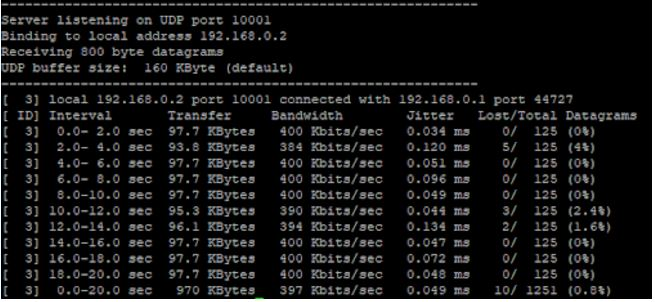
\includegraphics[width=0.9\columnwidth]{test/iperf_openvlc_originale} 
    \caption{Test iperf riportato nella documentazione di OpenVLC}
    \label{fig:iperf_openvlc_originale}
\end{figure}

\noindent In figura \ref{fig:iperf_openvlc_luce_ambiente}, si riporta il test iperf svolto in ambiente luminoso con OpenVLC originale. Si osserva che le differenze rispetto al test illustrato precedentemente, non sono statisticamente significative.
\begin{figure}[H] 
    \centering 
    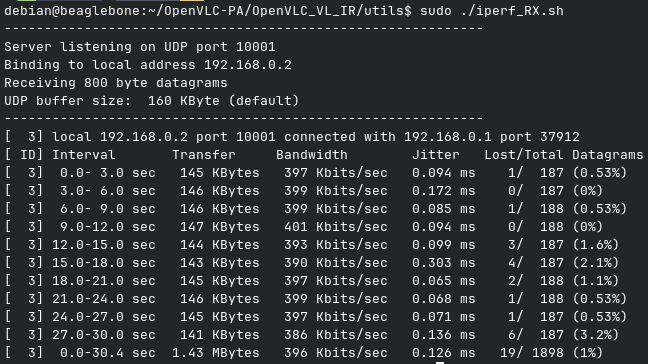
\includegraphics[width=0.9\columnwidth]{test/master_luce_ambiente} 
    \caption{Test iperf con OpenVLC in ambiente luminoso}
    \label{fig:iperf_openvlc_luce_ambiente}
\end{figure}

\noindent In figura \ref{fig:iperf_openvlc_auth_luce_ambiente}, si riporta il test iperf svolto in ambiente luminoso con OpenVLC e con l'utilizzo del modulo di autenticazione sviluppato.
\begin{figure}[H] 
    \centering 
    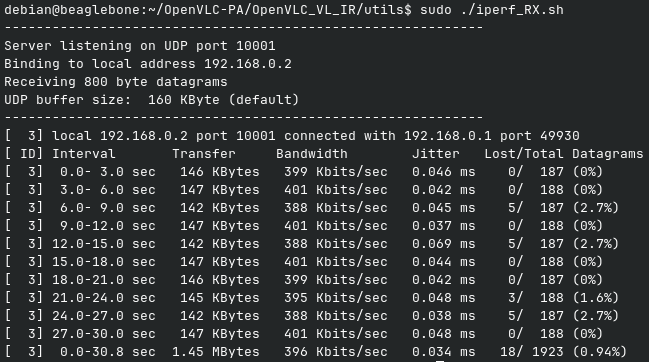
\includegraphics[width=0.9\columnwidth]{test/PhyAuth_luce_ambiente} 
    \caption{Test iperf con OpenVLC e modulo di autenticazione in ambiente luminoso}
    \label{fig:iperf_openvlc_auth_luce_ambiente}
\end{figure}

\noindent In figura \ref{fig:iperf_openvlc_auth_buio}, si riporta il test iperf svolto in ambiente buio con OpenVLC e con l'utilizzo del modulo di autenticazione sviluppato.
\begin{figure}[H] 
    \centering 
    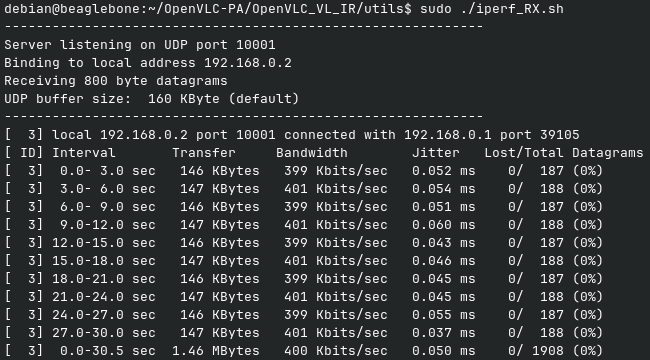
\includegraphics[width=0.9\columnwidth]{test/PhyAuth_buio} 
    \caption{Test iperf con OpenVLC e modulo di autenticazione in ambiente buio}
    \label{fig:iperf_openvlc_auth_buio}
\end{figure}

\noindent In figura \ref{fig:iperf_openvlc_auth_luce_disturbo}, si riporta il test iperf svolto in ambiente luminoso con OpenVLC e con l'utilizzo del modulo di autenticazione sviluppato. In più, in questo test è stato introdotto un disturbo luminoso, posizionando una lampada diretta verso il fotodiodo ricevitore ad una distanza di circa 20 centimetri. Tale disturbo è stato indotto per simulare un attacco di disturbo alla comunicazione, in modo tale da testare la robustezza della comunicazione.
\begin{figure}[H] 
    \centering 
    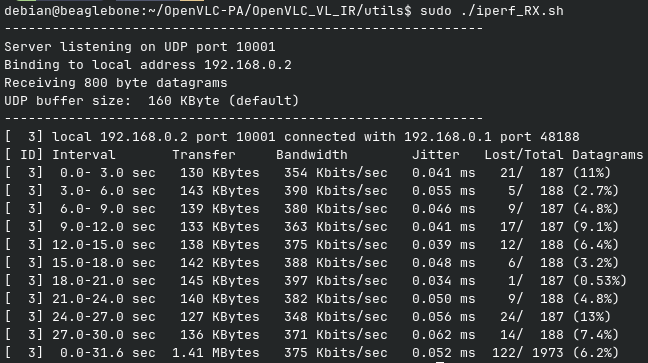
\includegraphics[width=0.9\columnwidth]{test/PhyAuth_luce_e_disturbo} 
    \caption{Test iperf con OpenVLC e modulo di autenticazione in ambiente luminoso con disturbo indotto}
    \label{fig:iperf_openvlc_auth_luce_disturbo}
\end{figure}

\subsection{Analisi dei risultati}

Nella seguente tabella si riassumono i risultati dei test descritti nella precedente sezione. I dati sono ricavati dall'ultima riga di ogni test, che rappresenta il valore medio delle metriche calcolate nell'intervallo di tempo in cui si è svolta la comunicazione.
\begin{table}[H]
    \caption{Tabella riassuntiva dei risultati dei test sul modulo di autenticazione}
    \label{tab:riass-test-auth}
    \resizebox{\textwidth}{!}{%
        \begin{tabular}{llllll}
            \hline
            \textbf{Test} & \textbf{Interval} & \textbf{Transfer} & \textbf{Bandwidth} & \textbf{Jitter} & \textbf{Lost/Total}\\
            \hline
            OpenVLC\\in ambiente\\luminoso & 30.4 sec & 1.43 MBytes & 396 Kbits/sec & 0.126 ms & 19/1898 (1\%) \\
            \hline
            OpenVLC\\+ modulo\\in ambiente\\luminoso & 30.8 sec & 1.45 MBytes & 396 Kbits/sec & 0.034 ms & 18/1923 (0.94\%) \\
            \hline
            OpenVLC\\+ modulo\\in ambiente\\buio & 30.5 sec & 1.46 MBytes & 400 Kbits/sec & 0.050 ms & 0/1988 (0\%) \\
            \hline
            OpenVLC\\+ modulo\\in ambiente\\luminoso\\con disturbo & 31.6 sec & 1.41 MBytes & 375 Kbits/sec & 0.052 ms & 122/1973 (6.2\%) \\
            \hline
        \end{tabular}
    }
\end{table}

\noindent Come si può osservare dalle prime due righe della tabella \ref{tab:riass-test-auth}, a parità di condizioni ambientali, non c'è alcuna differenza sistematicamente significativa tra le prestazioni del sistema con e senza l'utilizzo del modulo di autenticazione. Le lievi differenze presenti sono infatti da interpretarsi come rumore. Di conseguenza si può affermare che la sua introduzione non ha un impatto rilevante sulle prestazioni del sistema.

Si possono invece notare differenze significative tra i test svolti in ambiente luminoso e quelli svolti in diverse condizioni di luminosità.\\
In particolare, il test svolto in ambiente buio ha mostrato un'ampiezza di banda (bandwidth) e un tasso di perdita migliori rispetto a quelli svolti in ambiente luminoso. Questo suggerisce che la comunicazione tramite luce visibile, seppure in maniera minima, trattandosi di una variazione dell'1\%, è sicuramente influenzata dalla presenza di luce ambientale.\\
Inoltre, il test svolto in ambiente luminoso con disturbo indotto ha mostrato un tasso di perdita notevolmente più alto rispetto agli altri test, pari al 6.2\%. Si deduce che la presenza di fonti luminose dirette in direzione del fotodiodo ricevitore, sia in grado di disturbare notevolmente la comunicazione. Tuttavia è importante evidenziare che la situazione in cui è stato testato il sistema, e cioè posizionando una fonte luminosa a distanza molto ravvicinata al fotodiodo, è estrema. Di conseguenza, resta particolarmente difficoltoso, per un potenziale attaccante che volesse disturbare la ricezione dei dati, farlo in questa maniera.

% ================================================================= %
\section{Test su OpenVLC}
In questa sezione si riportano i risultati dei test svolti sul \textit{framework} OpenVLC originale, cioè senza l'utilizzo del modulo di autenticazione sviluppato. L'obbiettivo di questi test è quello di analizzare le prestazioni di OpenVLC a diverse distanze ed inclinazioni.

Sono stati condotti nove test, in ognuno dei quali sono stati trasmessi 1000 pacchetti di dati tramite il comando \texttt{nc} (netcat), ognuno della dimensione di 1480 byte. In tutti i test il \textit{payload} era formato da byte "FF", ovvero da 8 bit impostati a "1", in modo tale da poter individuare efficacemente eventuali bit corrotti. L'unica eccezione è il test denominato "50 cm bit-0", in cui il \textit{payload} era formato da byte "00", ovvero da 8 bit impostati a "0", per poter osservare eventuali bias a favore di bit-0 piuttosto che bit-1.

Tutti i test sono stati svolti in ambiente luminoso e senza l'utilizzo di Reed-Solomon, in modo tale da poter osservare le prestazioni del canale fisico senza l'intervento di alcun protocollo di correzione degli errori.

Inoltre, c'è da precisare che le schede BeagleBone non dispongono di una capacità computazionale elevata, di conseguenza il solo fatto di osservare la comunicazione e salvarne i dati, rende le schede maggiormente soggette ad errori. Questo implica che le metriche di errore calcolate durante i test sono sovrastimate rispetto a quelle che il sistema raggiunge in condizioni normali.\\

\noindent I test vengono valutati utilizzando le seguenti metriche:
\begin{itemize}
    \item \gls{ber}\glsfirstoccur: rapporto tra il numero di bit ricevuti in errore e il numero totale di bit trasmessi, indicativo dell’affidabilità a livello fisico del canale;
    \item Percentuale di byte corrotti: percentuale di byte che contengono almeno un bit errato rispetto al totale dei byte trasmessi, utile per valutare la possibilità di correggere errori con Reed-Solomon;
    \item \gls{prr}\glsfirstoccur: frazione di pacchetti correttamente ricevuti sul numero di pacchetti inviati, misura l’efficacia complessiva del link;
    \item \gls{plr}\glsfirstoccur: percentuale di pacchetti persi rispetto al totale inviato; è il complementare di \gls{prr};
    \item Percentuale di \textit{payload} ricevuto: rapporto tra il numero di byte di \textit{payload} validi ricevuti e il numero di byte di \textit{payload} trasmessi, espressa in percentuale, per quantificare l’efficienza utile della trasmissione.
\end{itemize}

\subsection{Data collection}
Come accennato in precedenza, sono stati condotti nove test, tutti in ambiente luminoso.

L'unico test in cui il \textit{payload} era formato da byte "00" è il test denominato "50 cm bit-0", in cui le schede sono state posizionate una di fronte all'altra ad una distanza di 50 centimetri. In tutti gli altri il \textit{payload} era formato da byte "FF".

Nei test denominati "50 cm bit-1", "100 cm", "150 cm", "200 cm", le schede sono state posizionate perfettamente allineate una di fronte all'altra ad una distanza di 50, 100, 150 e 200 centimetri rispettivamente.

Nei test denominati "50 cm 10°", "50 cm 45°", "50 cm 60°", "50 cm 90°", le schede sono state posizionate ad una distanza di 50 centimetri, ma con un'inclinazione di 10°, 45°, 60° e 90° rispettivamente. Ovvero per ogni inclinazione, la scheda trasmittente è stata ruotata, rispetto alla scheda ricevente, di un angolo corrispondente, mantenendo la stessa distanza.

\subsection{Analisi dei risultati}
\subsubsection{Bias a favore di bit-0}
Per prima cosa, è necessario confrontare i test "50 cm bit-0" e "50 cm bit-1", in modo tale da osservare se vi è un bias a favore di bit-0 rispetto a bit-1. In tabella \ref{tab:bit-bias} sono riportate le metriche di errore calcolate per i due test.

Nonostante, a prima vista, la differenza in tutte le metriche sembrerebbe minima, è importante considerare che la numerosità dei campioni è di diversi milioni di bit. Di conseguenza, anche una piccola differenza può essere considerata statisticamente significativa.

Si osserva che le uniche metriche che non presentano una differenza significativa sono il \gls{prr} e il \gls{plr}. Il che denota, come ci si aspetterebbe date le pari condizioni ambientali in cui sono stati svolti i test, che in entrambi i casi le schede riescono a sincronizzarsi correttamente.

Tuttavia, si osserva che il \gls{ber} è più basso per i bit-0 rispetto ai bit-1, con un valore di 1.10\% per i bit-0 e di 1.25\% per i bit-1. Inoltre, la percentuale di byte corrotti è più alta per i bit-1 (2.56\%) rispetto ai bit-0 (1.93\%). Infine, la percentuale di \textit{payload} ricevuto è più alta per i bit-0 (99.24\%) rispetto ai bit-1 (95.83\%). Questo indica che i bit-1 tendono a essere corrotti più frequentemente rispetto ai bit-0, il che suggerisce un bias a favore dei bit-0.

La presenza di questo bias comporta che le metriche di errore calcolate per i successivi test, in quanto basati su bit-1, sono da considerarsi sovrastimate. In una normale comunicazione, ci si aspetta un bilanciamento tra i bit-0 e i bit-1, e di conseguenza che le metriche di errore siano comprese tra i valori di errore dei bit-0 e dei bit-1 qui presentati.

\begin{table}[H]
    \caption{Confronto delle metriche di errore di bit-0 e bit-1: bias a favore di bit-0}
    \label{tab:bit-bias}
    \begin{tabularx}{\textwidth}{Xll}
        \hline
        \textbf{Metrica} & \textbf{50 cm bit-0} & \textbf{50 cm bit-1}\\
        \hline
        Bit Error Ratio (\gls{ber})            & 1.10\%  & 1.25\% \\
        \hline
        \% Byte corrotti                & 2.56\%  & 1.93\% \\
        \hline
        Packet Reception Rate (\gls{prr})     & 93.80\% & 93.90\% \\
        \hline
        Packet Loss Rate (\gls{plr})          & 6.20\%  & 6.10\% \\
        \hline
        \% Payload Ricevuto             & 99.24\% & 95.83\% \\
        \hline
    \end{tabularx}
\end{table}

\subsubsection{Test in diverse posizioni}
Testando la comunicazione in diverse posizioni, si è osservato che, come ci si aspetterebbe, all'aumentare della distanza e dell'inclinazione tra le schede, tutte le metriche di errore tendono a peggiorare.

In figura \ref{fig:ber_distanze} si riporta il \gls{ber} in funzione della distanza tra le schede. Si osserva una progressiva degradazione della qualità della comunicazione ed un'accelerazione nel tasso di errore a partire dai 100 centimetri.

\begin{figure}[H] 
    \centering 
    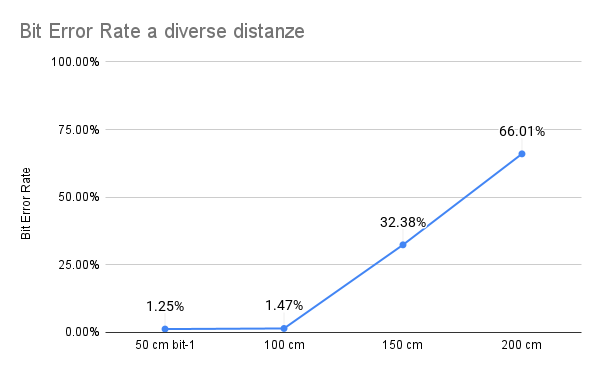
\includegraphics[width=0.9\columnwidth]{test/ber_distanze} 
    \caption{Test Bit Error Ratio (\gls{ber}) in funzione della distanza}
    \label{fig:ber_distanze}
\end{figure}

Analogamente, in figura \ref{fig:ber_inclinazioni} si riporta il \gls{ber} in funzione dell'inclinazione tra le schede. Anche in questo caso si osserva una degradazione della comunicazione all'aumentare dell'inclinazione, con un tasso di errore che cresce in maniera esponenziale a partire dai 60°.

È interessante notare che, anche ad un'inclinazione ampia come 60°, il BER è comunque limitato. Il che suggerisce che, contrariamente a quanto si potrebbe pensare, la comunicazione tramite luce visibile non sia strettamente unidirezionale, rendendo possibile l'intercettazione del segnale anche da posizioni angolate.\\
Tuttavia, bisogna considerare che i test sono stati svolti ad una distanza limitata, e che combinata a distanze maggiori, l'inclinazione ha sicuramente un impatto negativo sulla comunicazione. Inoltre, come dimostrano i test successivi, all'aumentare dell'inclinazione, corrisponde un aumento del \gls{plr}, il che renderebbe difficoltosa un'intercettazione esaustiva del segnale ad alte inclinazioni.

\begin{figure}[H] 
    \centering 
    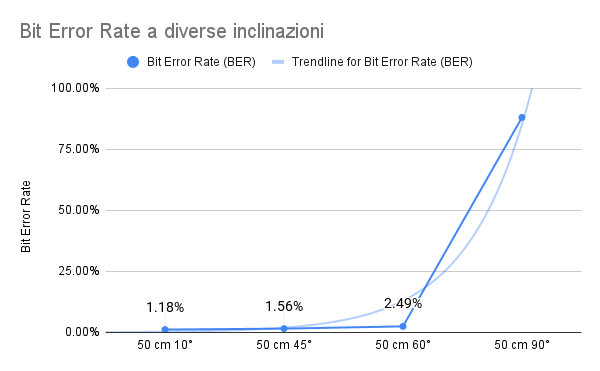
\includegraphics[width=0.9\columnwidth]{test/ber_inclinazioni} 
    \caption{Test Bit Error Ratio (\gls{ber}) in funzione dell'inclinazione}
    \label{fig:ber_inclinazioni}
\end{figure}

In figura \ref{fig:prr_distanze} si riporta il \gls{prr} e la percentuale di \textit{payload} ricevuto in funzione della distanza tra le schede. Si osserva un graduale peggioramento in entrambe le metriche. Si deduce che, all'aumentare della distanza, aumenta sia la perdita di interi pacchetti, sia la perdita di dati all'interno dei pacchetti stessi. 

\begin{figure}[H] 
    \centering 
    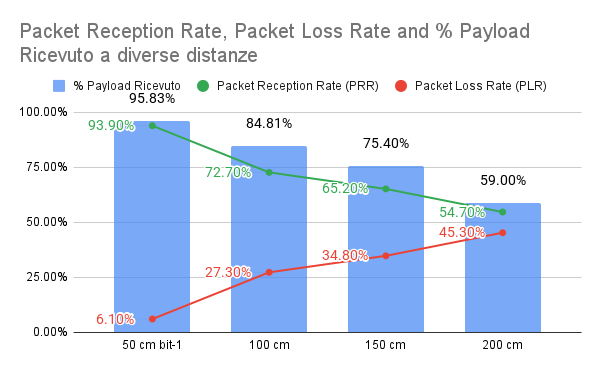
\includegraphics[width=0.9\columnwidth]{test/prr_distanze} 
    \caption{Test Packet Reception Rate (\gls{prr}) in funzione della distanza}
    \label{fig:prr_distanze}
\end{figure}

Analogamente, in figura \ref{fig:prr_inclinazioni} si riporta il \gls{prr} e la percentuale di \textit{payload} ricevuto in funzione dell'inclinazione tra le schede. Anche in questo caso si possono fare le medesime considerazioni fatte per i test in funzione della distanza.

\begin{figure}[H] 
    \centering 
    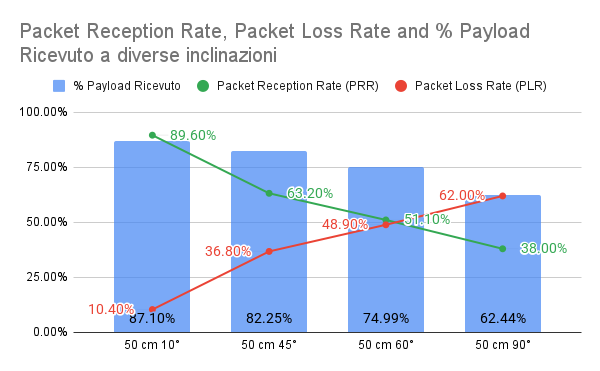
\includegraphics[width=0.9\columnwidth]{test/prr_inclinazioni} 
    \caption{Test Packet Reception Rate (\gls{prr}) in funzione dell'inclinazione}
    \label{fig:prr_inclinazioni}
\end{figure}

In figura \ref{fig:rs_distanze} si riporta la percentuale di byte corrotti in funzione della distanza tra le schede. Inoltre si riportano diversi valori di Reed-Solomon, in modo tale da poter individuare, per ogni distanza, la presenza di un valore di Reed-Solomon che permetta di correggere gli errori a quella distanza.

Ogni valore di Reed-Solomon è indicato da RS(n,k), dove n è il numero di byte totali (informativi + codici di correzione) e k è il numero di byte informativi. Ad esempio RS(15,2) indica un codice Reed-Solomon che per ogni 2 byte di informazione trasmessi, aggiunge 13 byte di codici di correzione, per un totale di 15 byte.\\
Ogni valore di Reed-Solomon è graficamente rappresentato da una \textit{stepped area}, in cui la parte inferiore rappresenta la percentuale di byte che è in grado di correggere. In particolare, sono riportati cinque possibili valori di Reed-Solomon (in ordine di capacità di correzione): RS(15,2), RS(15,4), RS(15,7), RS(15,11) e RS(216,200).\\
Il valore supportato nativamente da OpenVLC è RS(216,200). Gli altri valori sono stati scelti in quanto sono i più diffusi, nonché quelli indicati dallo standard IEEE 802.15.7 per questo tipo di comunicazione\\
Naturalmente, ad una maggiore capacità di correzione corrisponderebbe inevitabilmente un rallentamento nella comunicazione, in quanto si dovrebbero trasmettere più byte di codici di correzione.

Come si può vedere, la percentuale di byte corrotti rispecchia il \gls{ber} e, per distanze fino a 100 centimetri, rientra nelle capacità di correzione di RS(216,200). Questo significa che, come si può osservare empiricamente, a quelle distanze c'è una perdita di informazione molto bassa o addirittura nulla.

\begin{figure}[H] 
    \centering 
    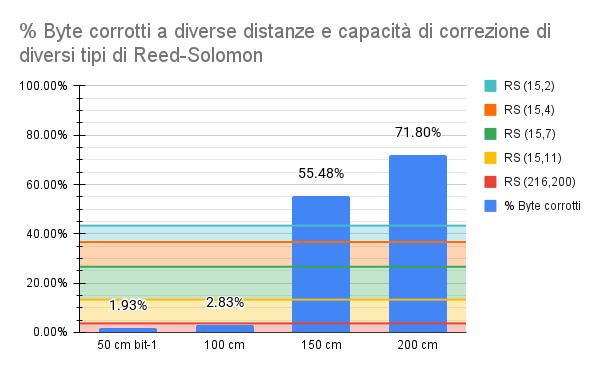
\includegraphics[width=0.9\columnwidth]{test/rs_distanze} 
    \caption{Test sulla percentuale di byte corrotti in funzione della distanza}
    \label{fig:rs_distanze}
\end{figure}

Analogamente, in figura \ref{fig:rs_inclinazioni} si riporta la percentuale di byte corrotti in funzione dell'inclinazione tra le schede. Anche in questo caso si osserva che, fino ad un'inclinazione di 45°, la percentuale di byte corrotti rientra nelle capacità di correzione di RS(216,200). Tuttavia, si può notare che ad una distanza di 60°, per poter garantire la piena correzione degli errori, sarebbe necessario utilizzare un valore di Reed-Solomon più robusto, ad esempio RS(15,11). All'inclinazione di 90°, invece, la percentuale di byte corrotti è tale da non poter essere corretta da alcun valore di Reed-Solomon qui riportato.

\begin{figure}[H] 
    \centering 
    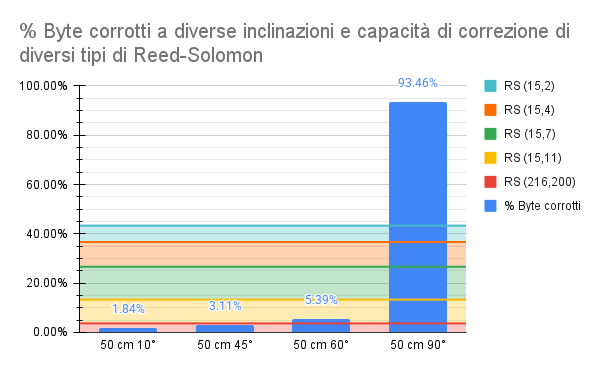
\includegraphics[width=0.9\columnwidth]{test/rs_inclinazioni} 
    \caption{Test sulla percentuale di byte corrotti in funzione dell'inclinazione}
    \label{fig:rs_inclinazioni}
\end{figure}